\section*{Methods}
RF pulses were designed for the 24-channel loop transmit array (Figure \ref{fig:Coil}) that will be built for the MRCoG scanner  and compressed to 16 channels using array compressed parallel transmission \cite{cao2016array}. $B_1^+$ maps used in the pulse design were simulated in a human head model using Ansys High Frequency Structure Simulator (Canonsburg, PA, USA) with 1.5 mm isotropic resolution. A SPINS  trajectory \cite{malik2012tailored} (Figure \ref{fig:Target}a\&b) with 5 mm max resolution was empirically designed for the pulse. The gradient duration was minimized to 10 ms through time-optimal design \cite{lustig2008fast} subject to the proposed MRCoG scanner’s gradient amplitude and slew rate constraints of 200 mT/m and 700T/m/s, respectively. 

\begin{figure}
	\centering
	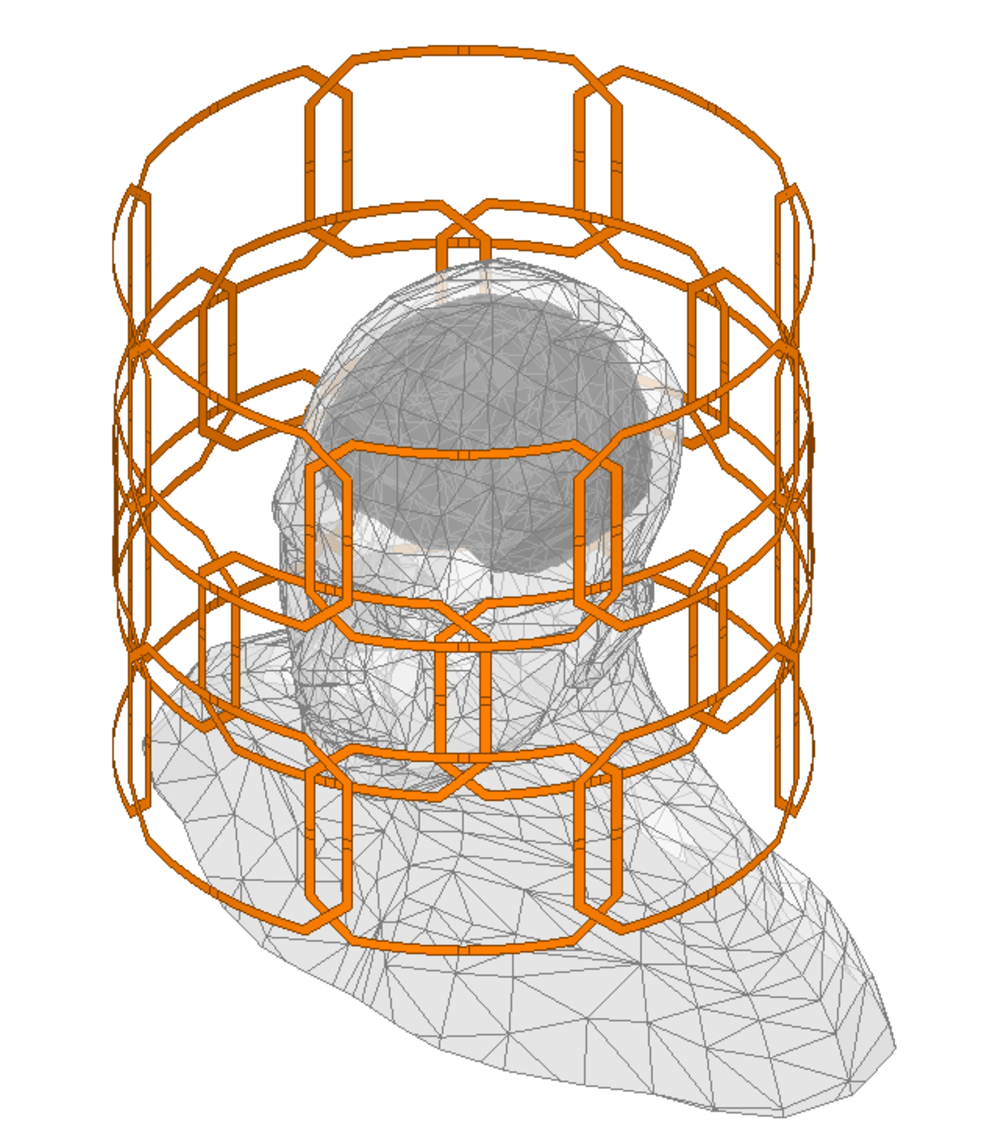
\includegraphics[width=3cm]{kspace_PTX_Coil}
	\caption{24-channel loop Tx array. The array has diameter 32 cm and height 28 cm. The 16 cm $times$ 11 cm loops are arranged in 3 rows of 8.}
	\label{fig:Coil}
\end{figure}



\begin{figure}
	\centering
	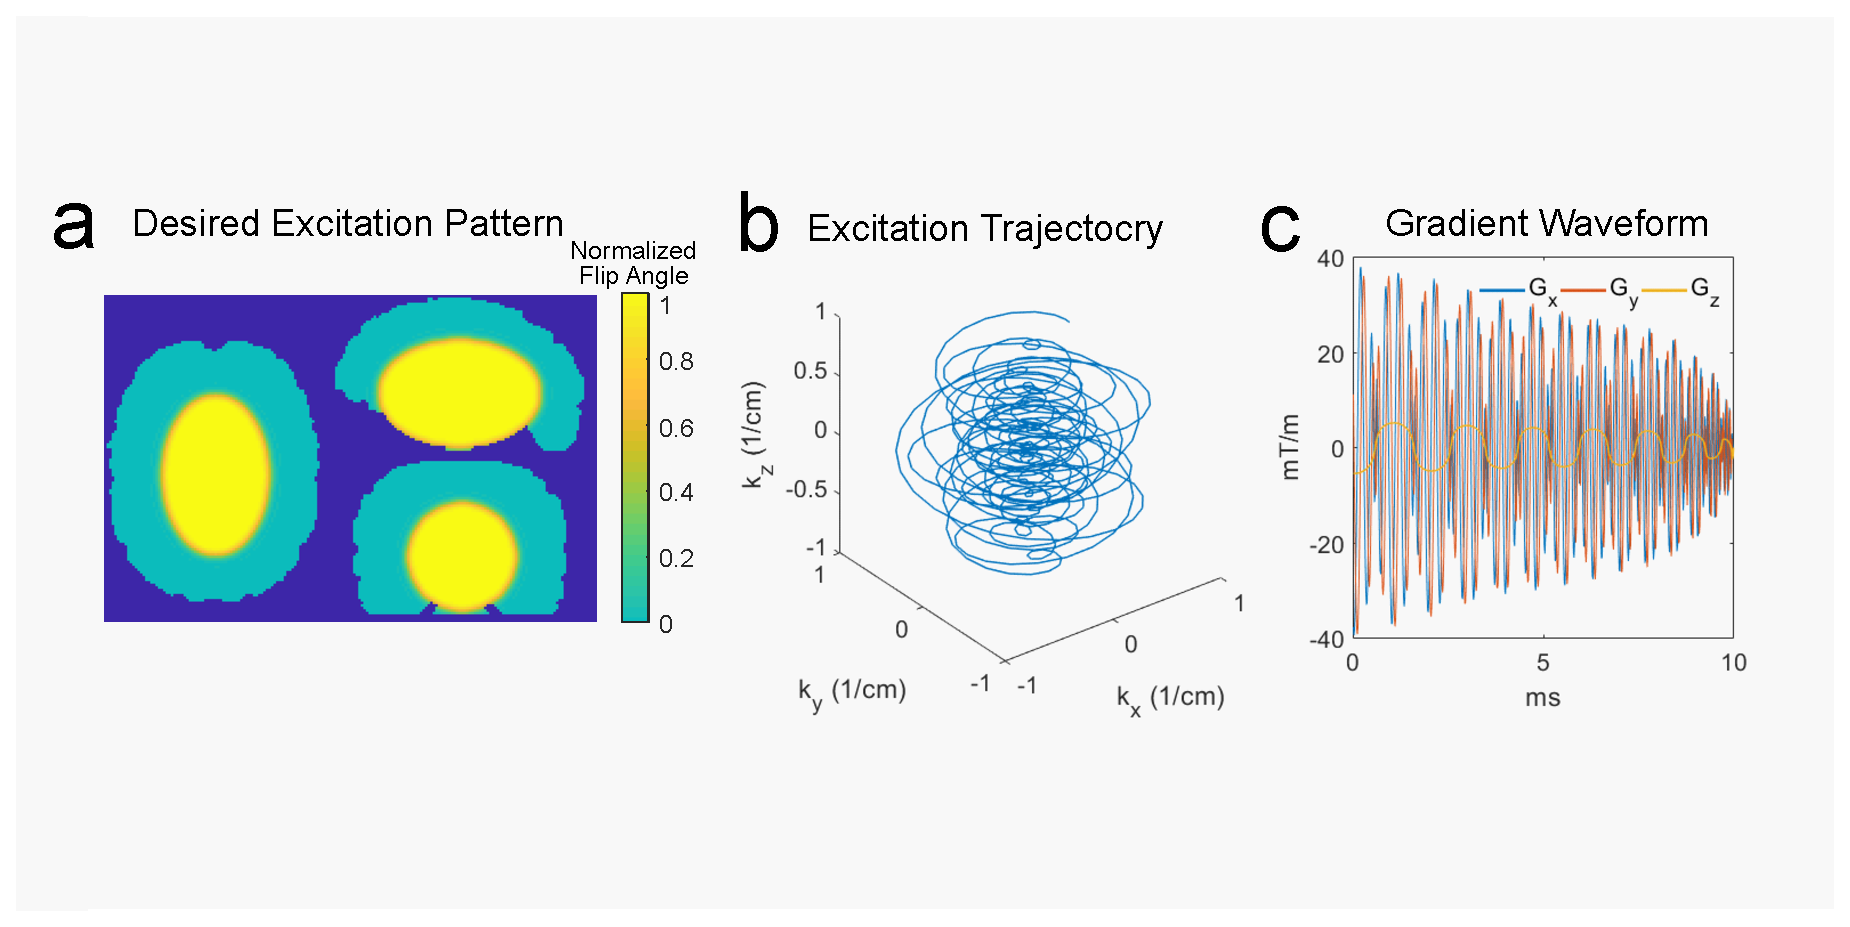
\includegraphics[width=\textwidth]{kSpace_PTX_Pattern_Trajectory}
	\caption{(a) Target excitation pattern for the IVS pulses. (b) 10 ms SPIN trajectory used in the designs. (c) Gradient waveforms of the excitation trajectory.}
	\label{fig:Target}
\end{figure}
Figure \ref{fig:Target}a shows the target pattern for the pulse design shaped as an ellipse centered on the ventricles with AP/HF/LR semi-axes of 4.8/3.2/3.2 cm. The target pattern was smoothed by a Fermi filter. Pulses were designed to excite the entire ellipse and achieve zero excitation in voxels in the cerebrum but outside the ellipse. Both the smoothed target pattern and the $B_1^+$ maps were undersampled from 128$\times$128$\times$96 grids (1.5mm iso-resolution) into 64$\times$64$\times$48 grids (3mm iso-resolution). The RF designs were done with the 64$\times$64$\times$48 grid size. The resulted pulses were evaluated against the target pattern with the 128$\times$128$\times$96 grid in order to expose Gibbs ringing. The normalized root-mean-square error (NRMS) was calculated against the voxels within the cerebrum.

With conventional spatial domain design, RF pulses were solved using an iterative least-squares conjugate-gradient decent method \cite{Grissom:2006:MRM}. With the proposed k-space domain design, RF pulses were solved with different parallelization parameters: thread number, patch width, and inclusion width. In order to study the computational acceleration provided by parallel computing, the design problem was solved with thread numbers ranging from 1 to 32, while the patch width and inclusion width were both set to 4. In order to study the computation time and error with respect to different patch widths and inclusion widths, we then held the computing threads constant at 16 while varying the patch and inclusion widths. The computation was done on a computer with a 512 GB RAM and two 24-core 2.1 GHz Intel Xeon CPUs which provides maximum 94 threads. For each design case, the computation was run 5 times, and the mean computation time and the NRMSE were recorded.

In order to demonstrate the k-space domain design’s robustness to Gibbs ringing, the target pattern and $B1^+$ maps were down-sampled into 32$\times$32$\times$24 (6mm iso-resolution)  and 64$\times$64$\times$48 grids (3mm iso-resolution). The outer sections of the excitation trajectory, equaling 2.1 ms, was excluded so that the maximum excitation resolution matched with the chosen 6 mm iso-resolution. All three designs were evaluated against the target pattern with the fully sampled 128$\times$128$\times$96 grid for validation.

The k-space domain design method's performance regarding k-space undersampling, which is desired for shorter pulse duration, was also examined and compared against the spatial domain design. The undersampling was achieved by reducing the numbers of the previously specified SPIN trajectory's polar and azimuthal rotations proportionally by a factor called acceleration factor, as shown in the third row of Figure \ref{fig:kspace_PTX_Acceleration}.    

In order to show the k-space domain design method's ability to compensate moderate off-resonance and compare it against the spatial domain method. We incorporated a normalized field map with Gaussian inhomogeneity centered above the frontal sinus (Figure \ref{fig:kspace_PTX_B0}a), mimicking a characteristic susceptibility induced $B_0$ inhomogeneity. The field maps were than scaled so that the maximum off-resonance reached +100 Hz, +200 Hz, and +300 Hz. Off-resonance corrected spatial domain designs were done with system matrices whose field maps were also incorporated through time segmentation approximation \cite{fessler2005toeplitz}. k-space domain design were done with or without off-resonance correction.